\documentclass[svgnames,tikz]{standalone}
\usetikzlibrary{positioning,arrows}

\tikzset{
  focus/.style args={#1 at #2}{
    insert path={
      %{ [white] (#2.north east) rectangle (#2.south west)}
      ($(#2.center)!#1!(#2.north east) $) rectangle ($(#2.center)!#1!(#2.south west) $)
    }
  },
  focusout/.style args={#1 at #2}{
    even odd rule,
    insert path={
      (#2.north east) rectangle (#2.south west)
      ($(#2.center)!#1!(#2.north east) $) rectangle ($(#2.center)!#1!(#2.south west) $)
    }
  },
  txt/.style={font=\Large\tt},
  img/.style={
     inner sep=2pt,
     draw,
     label/.append style={font=\small\tt},
  },
}


\begin{document}
\begin{tikzpicture}
\tikzset{every node/.style={node distance=5pt, font=\Huge}}

\node[txt] (p0) {\rlap{clip(}\phantom{filter(}}; %% for alignment

\node[img, yslant=.5] (p1) [right=of p0] { 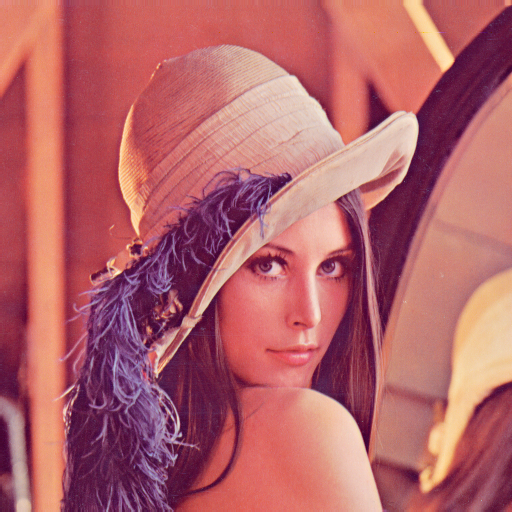
\includegraphics[width=2cm]{../images/lena_color.png} };

\node[txt] (p2) [right=of p1.west -| p1.east] { , };

\node[txt] (p2) [right=of p2, font=\normalsize, text width=3.5cm] {DiamondShape\_ROI};

\node[txt] (p2) [right=of p2] { ) $\rightarrow$ };

\node[] (p3) [right=of p2] {
  \begin{tikzpicture}
    \begin{scope}
      \clip (0,1) -- (-1,0) -- (0,-1) -- (1,0) -- cycle;
      \node[anchor=center] at (0,0) { 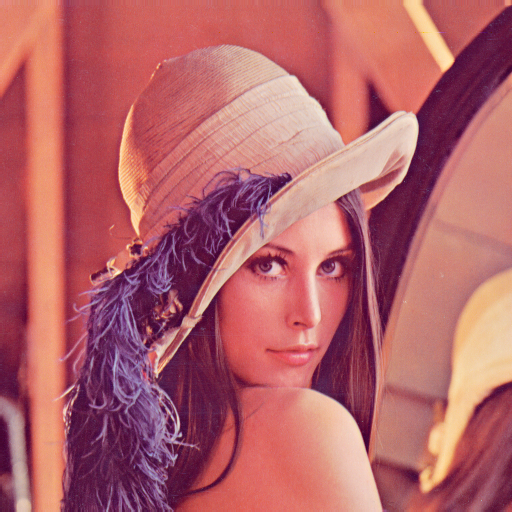
\includegraphics[width=3cm]{../images/lena_color.png} };
    \end{scope}

    \draw (0,1) -- (-1,0) -- (0,-1) -- (1,0) -- cycle;
  \end{tikzpicture}
};

\end{tikzpicture}
\end{document}
